\section{线性表 (Linear  List)}

\begin{frame}[fragile]
  \frametitle{线性表 --- Linear  List}
  \begin{enumerate}
  \item 基本概念
  \item 顺序表
  \item 链表
  \end{enumerate}
\end{frame}

\subsection{线性表概述}
\begin{frame}[fragile]
  \frametitle{线性表}

  \begin{easylist}
    & 线性表举例:
    && 英文字母表 $A, B, C, \cdots, Z$
    && 某单位近5年的计算机数量 $(40, 60, 100, 150, 180)$
    && 某产品淘宝的销售记录.
    
    & 特点
    && 数据元素是多样的,但具有相同特性
    && 相邻元素之间有序偶关系<前驱, 后继>    
  \end{easylist}
\end{frame}

\begin{frame}[fragile]
  \frametitle{线性表}

  \begin{tcolorbox}[standard jigsaw, opacityback=0, colframe=red, title=线性表是n个数据元素的有限序列]
    \[
    (a_1, a_2, \cdots, a_i, \cdots, a_n)
    \]
  \end{tcolorbox}

  \begin{itemize}
  \item 存在唯一的{\color{red}第一个}数据元素,存在唯一的的{\color{red}最后一个}数据元素。
  \item 除第一个之外,每个数据元素只有一个前驱;除最后一个之外,每个数据元素只有
    一个后继。
  \item 线性表的长度:线性表中元素的个数,常记作length, len, n. 当空表时,len=0.
  \end{itemize}
\end{frame}

\begin{frame}[fragile]
  \frametitle{线性表的两种存储方式}
  \begin{enumerate}
  \item 方案1:顺序存储 --- 称顺序表
  \item 方案2:链式存储 --- 称链表
  \end{enumerate}
\end{frame}


\subsection{顺序表}
\begin{frame}[fragile]
  \frametitle{方案1: 顺序表 (Sequence List)}
  \begin{columns}
    \begin{column}[T]{.5\linewidth}
      \[
      (a_1, a_2, \cdots, a_i, \cdots, a_n)
      \]
      \begin{easylist}
        & 建一个数组, 用一组地址连续的存储单元依次存储数据元素。

        && 逻辑上相邻的数据元素,其物理存储位置也相邻

      \end{easylist}
    \end{column}
    \begin{column}[T]{.5\linewidth}
      \begin{tcolorbox}[]
        \scalebox{0.7}{
          \begin{tikzpicture}[scale=0.5, box/.style={draw, minimum width=1.2cm, minimum height=0.5cm, fill=yellow!10}]
	          \draw node[box] (a1) {$a_1$}
	          node[box, below=0 of a1] (a2) {$a_2$}
	          node[box, below=0 of a2] (a3) {$\cdots$}
	          node[box, below=0 of a3] (ai) {$a_i$}
	          node[box, below=0 of ai] (a5) {$\cdots$}
	          node[box, below=0 of a5] (an) {$a_n$}
	          node[box, below=0 of an, fill=gray!30] (a7) {}
	          node[box, below=0 of a7, fill=gray!30] (a8) {}
	          node[box, below=0 of a8, fill=gray!30] (a9) {};

	          \draw node[right=0.3 of a1] (p1) {$1$}
	          node[right=0.3 of a2] (p2) {$2$}
	          node[right=0.3 of ai] (pi) {$i$}
	          node[right=0.3 of an] (pn) {$n$}
	          node[right=0.3 of a7] (p7) {空闲}
	          node[right=0.3 of a8] (p8) {空闲}
	          node[right=0.3 of a9] (p9) {空闲};

	          \draw node[left=0.3 of a1] (p1) {$b$}
	          node[left=0.3 of a2] (p2) {$b+l$}
	          node[left=0.3 of ai] (pi) {$b+(i-1)\cdot l$}
	          node[left=0.3 of an] (pn) {$b+(n-1)\cdot l$}
	          node[left=0.3 of a7] (p7) {$b+n\cdot l$}
	          node[left=0.3 of a8] (p8) {$\cdots$}
	          node[left=0.3 of a9] (p9) {$b+(MaxLen-1)\cdot l$};

	          \draw node[above left=0.3 of p1] (tip) {起始地址/基地址};
	          \draw[draw=red, thick, -Latex] (tip) -> (p1);
          \end{tikzpicture}
        }
      \end{tcolorbox}
    \end{column}
  \end{columns}
\end{frame}

\begin{frame}[fragile]
  \frametitle{顺序表 (Sequence List)}
  \begin{columns}
    \begin{column}[T]{.5\linewidth}
      \begin{easylist}
        & 为便于维护处理,记录3个变量

        && 存放表元素的数组list;
        && 表的长度length;
        && 存储容量maxSize;

        & 常用的基本操作
        && 判断是否空: isEmpty()
        && 求长度: length()
        && 取元素: get(i)
        && 插入操作: insert(i,x)
        && 删除操作: remove(i)
        && 查找: indexOf(x)
        && 输出: display()
      \end{easylist}
    \end{column}
    \begin{column}[T]{.5\linewidth}
      \begin{tcolorbox}[]
        \scalebox{0.7}{
          \begin{tikzpicture}[scale=0.5, box/.style={draw, minimum width=1.2cm, minimum height=0.5cm, fill=yellow!10}]
	          \draw node[box] (a1) {$a_1$}
	          node[box, below=0 of a1] (a2) {$a_2$}
	          node[box, below=0 of a2] (a3) {$\cdots$}
	          node[box, below=0 of a3] (ai) {$a_i$}
	          node[box, below=0 of ai] (a5) {$\cdots$}
	          node[box, below=0 of a5] (an) {$a_n$}
	          node[box, below=0 of an, fill=gray!30] (a7) {}
	          node[box, below=0 of a7, fill=gray!30] (a8) {}
	          node[box, below=0 of a8, fill=gray!30] (a9) {};

	          \draw node[right=0.3 of a1] (p1) {$1$}
	          node[right=0.3 of a2] (p2) {$2$}
	          node[right=0.3 of ai] (pi) {$i$}
	          node[right=0.3 of an] (pn) {$n$}
	          node[right=0.3 of a7] (p7) {空闲}
	          node[right=0.3 of a8] (p8) {空闲}
	          node[right=0.3 of a9] (p9) {空闲};

	          \draw node[left=0.3 of a1] (p1) {$b$}
	          node[left=0.3 of a2] (p2) {$b+l$}
	          node[left=0.3 of ai] (pi) {$b+(i-1)\cdot l$}
	          node[left=0.3 of an] (pn) {$b+(n-1)\cdot l$}
	          node[left=0.3 of a7] (p7) {$b+n\cdot l$}
	          node[left=0.3 of a8] (p8) {$\cdots$}
	          node[left=0.3 of a9] (p9) {$b+(MaxLen-1)\cdot l$};
          \end{tikzpicture}
        }
      \end{tcolorbox}
    \end{column}
  \end{columns}
\end{frame}

\begin{frame}[fragile]
  \frametitle{补充:常用命名规则之驼峰与蛇形命名法}
  \begin{center}
    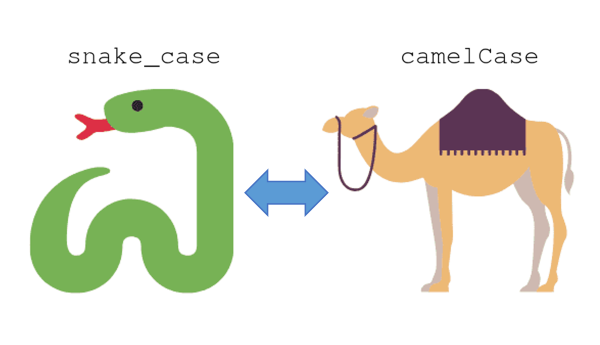
\includegraphics[width=0.5\textwidth]{figs/list/snake_case_camel_case.png}
    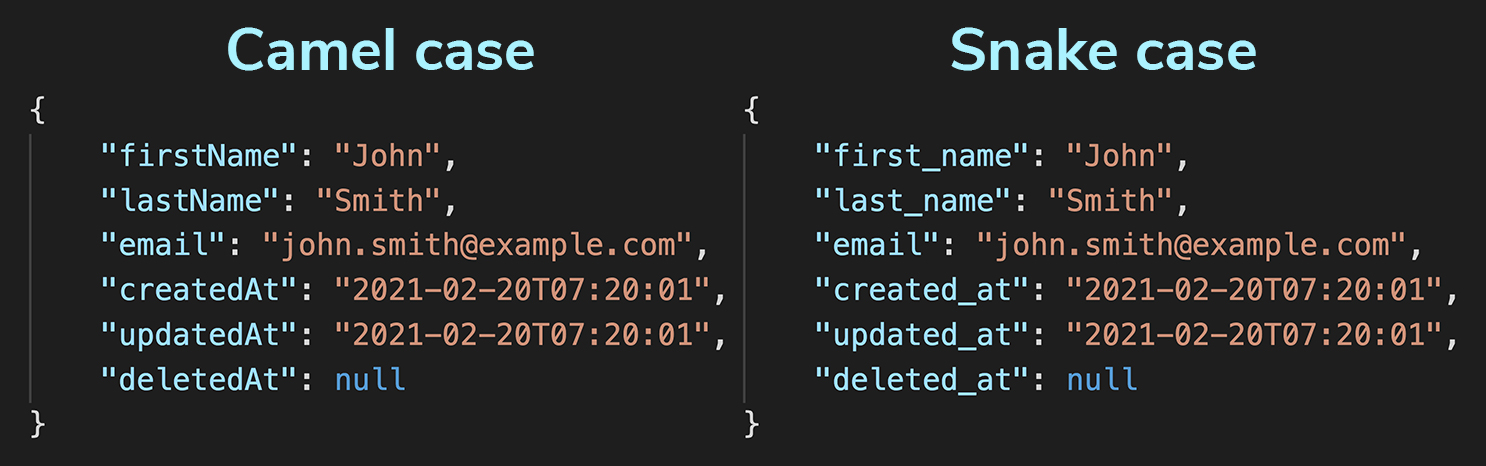
\includegraphics[width=0.85\textwidth]{figs/list/snake_vs_camel.jpg}
  \end{center}
\end{frame}

\begin{frame}[fragile]
  %\frametitle{线性表}
  \begin{minted}{java}
public class SequenceList {
    int maxSize; //最大长度
    int length; //当前长度
    Elem[] list; //对象数组

    public bool isEmpty()
    public int length()
    public Elem get(i) throws Exception
    public void insert(i,e)
    public void remove(i) throws Exception
    public int indexOf(e)
    public void display()
    public void clear()
}
  \end{minted}
\end{frame}

\begin{frame}[fragile]
  %\frametitle{线性表}
  \begin{minted}{python}
class SequenceList:
    def __init__(self, max_size, elements):
        self.max_size = max_size
        self.length = len(elements)
        self.elements = [0]*max_size
        for idx, value in enumerate(elements):
            self.elements[idx] = value

    def __len__(self):
        return self.length

    def __getitem__(self, i):
        return self.elements[i]

    def __setitem__(self, i, value):
        self.elements[i] = value

    def __delitem__(self, i):
        del self.elements[i]
        self.length = self.length - 1
  \end{minted}
\end{frame}

\begin{frame}[fragile]
  \frametitle{初始化顺序表}
  Java/C Example

  \begin{minted}{java}
//初始化空表
void initList(int size) {
    list = new Elem[size];
    maxSize = size; //初始存储容量
    length = 0; //空表长度为0
}
  \end{minted}

  Python Example:

  \begin{minted}{python}
    self.elements = [0]*max_size
  \end{minted}
\end{frame}

\begin{frame}[fragile]
  \frametitle{在index位置上插入元素e}
  \begin{minted}{java}
boolean insert(int index, Elem e) {
  if (length== maxSize)    //当前线性表已满
     {print("顺序表已满!");  return false;}
  if (index < 0 || index > length)    //插入位置编号不合法
    {print("参数错误!");  return false;}

  for (int j = length- 1; j >= index; j--)   //向后移动元素
     list[j + 1] = list[j];

  list[index] = e;    //插入元素
  length ++;
  return true;
}
  \end{minted}
\end{frame}


\begin{frame}[fragile]
  \frametitle{插入元素的时间复杂度}

  \scalebox{0.75} {
    \begin{tikzpicture}[box/.style={draw, minimum width=1.2cm, minimum height=0.65cm, fill=yellow!10}]
	    \draw node[box] (a1) {$a_1$}
	    node[box, right=0 of a1] (a2) {$a_2$}
	    node[box, right=0 of a2] (a3) {$\cdots$}
	    node[box, right=0 of a3] (a4) {$\cdots$}
	    node[box, right=0 of a4] (ai) {$a_i$}
	    node[box, right=0 of ai] (a6) {$\cdots$}
	    node[box, right=0 of a6] (a7) {$\cdots$}
	    node[box, right=0 of a7] (an) {$a_n$}
		  node[draw=red, ellipse, minimum width=0.65cm, minimum height=0.65cm, thick, fill=blue!10, below=0.5 of ai] (cur) {$e$};
		  \draw[draw = red, -Latex] (cur) -- (ai);
    \end{tikzpicture}
  }

  \begin{easylist}
    & 在长为n的线性表中插入一个元素,所需移动元素次数的平均次数为?

    && 有多少种可能的插入位置?$n+1$

    && 假设这些位置以同等概率出现,每个概率$\dfrac{1}{n+1}$。每个情形下分别移动
    $n, n-1, \cdots, 0$次。求加权和为$n/2$。

    && 平均时间复杂度:$T(n)=O(n)$
  \end{easylist}
\end{frame}

\begin{frame}[fragile]
  \frametitle{删除index位置上的元素}
  \scalebox{0.7}{
    \begin{tikzpicture}[scale=0.5, box/.style={draw, minimum width=1.2cm, minimum height=0.65cm, fill=yellow!10}]
	    \draw node[box] (a1) {$a_1$}
	    node[box, right=0 of a1] (a2) {$a_2$}
	    node[box, right=0 of a2] (a3) {$\cdots$}
	    node[box, right=0 of a3] (a4) {$\cdots$}
	    node[box, draw=red, thick, fill=red!20, right=0 of a4] (ai) {$a_i$}
	    node[box, right=0 of ai] (a6) {$\cdots$}
	    node[box, right=0 of a6] (a7) {$\cdots$}
	    node[box, right=0 of a7] (an) {$a_n$};
    \end{tikzpicture}
  }

  \begin{minted}{java}
boolean remove(int index) {
    if(index<0||index>=length)  
          return false;
    if(getLength()==0)
          return false;
    for (int j=index;j<length-1; j++)    //前移
          Elem[j]=elem[j+1];
    length--;
}
  \end{minted}
\end{frame}

\begin{frame}[fragile]
  \frametitle{删除元素的时间复杂度}
  \scalebox{0.7}{
    \begin{tikzpicture}[scale=0.5, box/.style={draw, minimum width=1.2cm, minimum height=0.65cm, fill=yellow!10}]
	    \draw node[box] (a1) {$a_1$}
	    node[box, right=0 of a1] (a2) {$a_2$}
	    node[box, right=0 of a2] (a3) {$\cdots$}
	    node[box, right=0 of a3] (a4) {$\cdots$}
	    node[box, draw=red, thick, fill=red!20, right=0 of a4] (ai) {$a_i$}
	    node[box, right=0 of ai] (a6) {$\cdots$}
	    node[box, right=0 of a6] (a7) {$\cdots$}
	    node[box, right=0 of a7] (an) {$a_n$};
    \end{tikzpicture}
  }

  \begin{itemize}
  \item 在长度为n的线性表中删除一个元素:
    \begin{itemize}
    \item 共有n个可能的位置,每个有1/n的概率。每个情形下分别移动n-1, …, 0次。求加权和为(n-1)/2。
    \item $T(n)=O(n)$
    \end{itemize}
  \end{itemize}

  \pause

  \begin{tcolorbox}[standard jigsaw, opacityback=0, colframe=red, title=结论]
    在顺序表中插入或删除一个元素时,平均移动一半元素,当$n$很大时,效率很低.
  \end{tcolorbox}
\end{frame}

\begin{frame}[fragile]
  \frametitle{顺序表特点:地址连续}
  \begin{columns}
    \begin{column}[T]{.5\linewidth}
      \begin{tcolorbox}[]
      \scalebox{0.7}{
        \begin{tikzpicture}[scale=0.5, box/.style={draw, minimum width=1.2cm, minimum height=0.5cm, fill=yellow!10}]
	        \draw node[box] (a1) {$a_1$}
	        node[box, below=0 of a1] (a2) {$a_2$}
	        node[box, below=0 of a2] (a3) {$\cdots$}
	        node[box, below=0 of a3] (ai) {$a_i$}
	        node[box, below=0 of ai] (a5) {$\cdots$}
	        node[box, below=0 of a5] (an) {$a_n$}
	        node[box, below=0 of an, fill=gray!30] (a7) {}
	        node[box, below=0 of a7, fill=gray!30] (a8) {}
	        node[box, below=0 of a8, fill=gray!30] (a9) {};

	        \draw node[right=0.3 of a1] (p1) {$1$}
	        node[right=0.3 of a2] (p2) {$2$}
	        node[right=0.3 of ai] (pi) {$i$}
	        node[right=0.3 of an] (pn) {$n$}
	        node[right=0.3 of a7] (p7) {空闲}
	        node[right=0.3 of a8] (p8) {空闲}
	        node[right=0.3 of a9] (p9) {空闲};

	        \draw node[left=0.3 of a1] (p1) {$b$}
	        node[left=0.3 of a2] (p2) {$b+l$}
	        node[left=0.3 of ai] (pi) {$b+(i-1)\cdot l$}
	        node[left=0.3 of an] (pn) {$b+(n-1)\cdot l$}
	        node[left=0.3 of a7] (p7) {$b+n\cdot l$}
	        node[left=0.3 of a8] (p8) {$\cdots$}
	        node[left=0.3 of a9] (p9) {$b+(MaxLen-1)\cdot l$};
        \end{tikzpicture}
      }
      \end{tcolorbox}
    \end{column}
    \begin{column}[T]{.5\linewidth}
      \begin{easylist}
        & 优点
        && 直观
        && 随机存储效率高
        \pause
        & 缺点
        && 移动元素代价大
      \end{easylist}
    \end{column}
  \end{columns}
\end{frame}


\subsection{链表}
\begin{frame}[fragile]
  \frametitle{方案2: 链式存储---链表}
  \begin{columns}
    \begin{column}[T]{.4\linewidth}
      \scalebox{0.5}{    \begin{tikzpicture}[fill=red, box/.style={draw, minimum width=2cm, minimum height=0.85cm, fill=yellow!10}]
	      \draw node[box] (dh) {数据域}  node[box, right=0 of dh] (ph) {指针域}
	 node[box, below=0.5 of dh] (d_li) {LI}  node[box, right=0 of d_li] (p_li) {43} node[left=0.2 of d_li] {1}
	 node[box, below=0.5 of d_li] (d_qian) {QIAN}  node[box, right=0 of d_qian] (p_qian) {13} node[left=0.2 of d_qian] {7}
	 node[box, below=0.5 of d_qian] (d_sun) {SUN}  node[box, right=0 of d_sun] (p_sun) {1} node[left=0.2 of d_sun] {13}
	 node[box, below=0.5 of d_sun] (d_wang) {WANG}  node[box, right=0 of d_wang] (p_wang) {?} node[left=0.2 of d_wang] {19}
	 node[box, below=0.5 of d_wang] (d_wu) {WU}  node[box, right=0 of d_wu] (p_wu) {37} node[left=0.2 of d_wu] {25}
	 node[box, below=0.5 of d_wu] (d_zhao) {ZHAO}  node[box, right=0 of d_zhao] (p_zhao) {7} node[left=0.2 of d_zhao] {31}
	 node[box, below=0.5 of d_zhao] (d_zheng) {ZHENG}  node[box, right=0 of d_zheng] (p_zheng) {?} node[left=0.2 of d_zheng] {37}
	 node[box, below=0.5 of d_zheng] (d_zhou) {ZHOU}  node[box, right=0 of d_zhou] (p_zhou) {25} node[left=0.2 of d_zhou] {43}
	node[box, minimum width=0.85cm, draw=red, fill=red!20, left=1 of d_li] (h) {31};

	\path[draw=red] (h.center) edge[out=270, in=155, -Latex, draw=red, thick] (d_zhao.west);
	\path[draw=blue] (p_zhao.east) edge[out=0, in=225, -Latex] (d_qian.west);
	\path[draw=blue] (p_qian.east) edge[out=0, in=225, -Latex] (d_sun.west);
	\path[draw=blue] (p_sun.east) edge[out=0, in=225, -Latex] (d_li.west);
\end{tikzpicture}

}
    \end{column}
    \begin{column}[T]{.6\linewidth}
      用一组任意的存储单元存储线性表的数据元素,利用指针指向直接后继的存储位置
    \end{column}
  \end{columns}
\end{frame}

\begin{frame}[fragile]
  \frametitle{单链表的类型定义}
  \begin{columns}
    \begin{column}[T]{.4\linewidth}
      \scalebox{0.5}{    \begin{tikzpicture}[fill=red, box/.style={draw, minimum width=2cm, minimum height=0.85cm, fill=yellow!10}]
	      \draw node[box] (dh) {数据域}  node[box, right=0 of dh] (ph) {指针域}
	 node[box, below=0.5 of dh] (d_li) {LI}  node[box, right=0 of d_li] (p_li) {43} node[left=0.2 of d_li] {1}
	 node[box, below=0.5 of d_li] (d_qian) {QIAN}  node[box, right=0 of d_qian] (p_qian) {13} node[left=0.2 of d_qian] {7}
	 node[box, below=0.5 of d_qian] (d_sun) {SUN}  node[box, right=0 of d_sun] (p_sun) {1} node[left=0.2 of d_sun] {13}
	 node[box, below=0.5 of d_sun] (d_wang) {WANG}  node[box, right=0 of d_wang] (p_wang) {?} node[left=0.2 of d_wang] {19}
	 node[box, below=0.5 of d_wang] (d_wu) {WU}  node[box, right=0 of d_wu] (p_wu) {37} node[left=0.2 of d_wu] {25}
	 node[box, below=0.5 of d_wu] (d_zhao) {ZHAO}  node[box, right=0 of d_zhao] (p_zhao) {7} node[left=0.2 of d_zhao] {31}
	 node[box, below=0.5 of d_zhao] (d_zheng) {ZHENG}  node[box, right=0 of d_zheng] (p_zheng) {?} node[left=0.2 of d_zheng] {37}
	 node[box, below=0.5 of d_zheng] (d_zhou) {ZHOU}  node[box, right=0 of d_zhou] (p_zhou) {25} node[left=0.2 of d_zhou] {43}
	node[box, minimum width=0.85cm, draw=red, fill=red!20, left=1 of d_li] (h) {31};

	\path[draw=red] (h.center) edge[out=270, in=155, -Latex, draw=red, thick] (d_zhao.west);
	\path[draw=blue] (p_zhao.east) edge[out=0, in=225, -Latex] (d_qian.west);
	\path[draw=blue] (p_qian.east) edge[out=0, in=225, -Latex] (d_sun.west);
	\path[draw=blue] (p_sun.east) edge[out=0, in=225, -Latex] (d_li.west);
\end{tikzpicture}

}
    \end{column}
    \begin{column}[T]{.6\linewidth}
      \begin{easylist}
        & 单链表:每个结点有一个指针域
        & 单链表可由头指针唯一确定,头指针指向第一个结点。
        & Java Code:

        \scriptsize

        \begin{minted}{java}
          class Node {
            Object data;
            Node next;
          }
        \end{minted}

      \end{easylist}
    \end{column}
  \end{columns}
\end{frame}

\begin{frame}[fragile]
  \frametitle{单链表的类型定义}
  \begin{columns}
    \begin{column}[T]{.4\linewidth}
      \scalebox{0.5}{    \begin{tikzpicture}[fill=red, box/.style={draw, minimum width=2cm, minimum height=0.85cm, fill=yellow!10}]
	      \draw node[box] (dh) {数据域}  node[box, right=0 of dh] (ph) {指针域}
	 node[box, below=0.5 of dh] (d_li) {LI}  node[box, right=0 of d_li] (p_li) {43} node[left=0.2 of d_li] {1}
	 node[box, below=0.5 of d_li] (d_qian) {QIAN}  node[box, right=0 of d_qian] (p_qian) {13} node[left=0.2 of d_qian] {7}
	 node[box, below=0.5 of d_qian] (d_sun) {SUN}  node[box, right=0 of d_sun] (p_sun) {1} node[left=0.2 of d_sun] {13}
	 node[box, below=0.5 of d_sun] (d_wang) {WANG}  node[box, right=0 of d_wang] (p_wang) {?} node[left=0.2 of d_wang] {19}
	 node[box, below=0.5 of d_wang] (d_wu) {WU}  node[box, right=0 of d_wu] (p_wu) {37} node[left=0.2 of d_wu] {25}
	 node[box, below=0.5 of d_wu] (d_zhao) {ZHAO}  node[box, right=0 of d_zhao] (p_zhao) {7} node[left=0.2 of d_zhao] {31}
	 node[box, below=0.5 of d_zhao] (d_zheng) {ZHENG}  node[box, right=0 of d_zheng] (p_zheng) {?} node[left=0.2 of d_zheng] {37}
	 node[box, below=0.5 of d_zheng] (d_zhou) {ZHOU}  node[box, right=0 of d_zhou] (p_zhou) {25} node[left=0.2 of d_zhou] {43}
	node[box, minimum width=0.85cm, draw=red, fill=red!20, left=1 of d_li] (h) {31};

	\path[draw=red] (h.center) edge[out=270, in=155, -Latex, draw=red, thick] (d_zhao.west);
	\path[draw=blue] (p_zhao.east) edge[out=0, in=225, -Latex] (d_qian.west);
	\path[draw=blue] (p_qian.east) edge[out=0, in=225, -Latex] (d_sun.west);
	\path[draw=blue] (p_sun.east) edge[out=0, in=225, -Latex] (d_li.west);
\end{tikzpicture}

}
    \end{column}
    \begin{column}[T]{.6\linewidth}
      \begin{easylist}
        & 单链表:每个结点有一个指针域
        & 单链表可由头指针唯一确定,头指针指向第一个结点。
        & Python Code:
        \scriptsize

        \begin{minted}{python}
          class Node:
            def __init__(self, data, next=None):
              self.data = data
              self.next = next

          first = Node(1)
          second = Node(2)
          last = Node(3)
          first.next=second
          second.next = last
          print(first.next.next.data)
        \end{minted}

      \end{easylist}
    \end{column}
  \end{columns}
\end{frame}

\begin{frame}[fragile]
  \frametitle{单链表上的常见操作}
  \begin{enumerate}
  \item 建立单链表create()
  \item 求表长length()
  \item 查找index(value)
  \item 插入insert(i,e)
  \item 删除remove(i)
  \item 获取元素get(index)
  \item 显示display()
  \end{enumerate}
\end{frame}

\begin{frame}[fragile]
  \frametitle{建立单链表}
  \begin{itemize}
  \item 链表是{\color{red}动态管理}的:链表中的每个结点占用的存储空间不是预先分
    配,而是运行时系统根据需求而生成的。
  \item 建立单链表从空表开始,每读入一个数据元素则申请一个结点,插入链表。
  \end{itemize}
\end{frame}

\begin{frame}[fragile]
  \frametitle{建立单链表:两种不同方式}
  如依次读入  25, 45, 18…

  \begin{columns}
    \begin{column}[T]{.5\linewidth}
      头部插入:

      \begin{tcolorbox}[]
        \scalebox{0.5}{
          \begin{tikzpicture}[fill=red, box/.style={draw, minimum width=0.85cm, minimum height=0.8cm, fill=red!5}]
	          \draw node[box] (h) {$\wedge$};

	          \draw node[box, below=0.5 of h] (h) {} node[box, right=of h] (d25) {25}  node[box, right=0 of d25] (p25) {$\wedge$};
	          \draw[draw, -Latex] (h.center) -- (d25);

	          \draw node[box, below=0.5 of h] (h) {}
            node[box, right=of h] (d45) {45}  node[box, right=0 of d45] (p45) {}
            node[box, right=of p45] (d25) {25}  node[box, right=0 of d25] (p25) {$\wedge$};
	          \draw[draw, -Latex] (h.center)  edge[-latex] (d45) (p45.center) -- (d25);

	          \draw node[box, below=0.5 of h] (h) {}
            node[box, right=of h] (d18) {18}  node[box, right=0 of d18] (p18) {}
            node[box, right=of p18] (d45) {45}  node[box, right=0 of d45] (p45) {}
            node[box, right=of p45] (d25) {25}  node[box, right=0 of d25] (p25) {$\wedge$};
	          \path[draw, -Latex] (h.center) edge[-latex] (d18) (p18.center)  edge[-latex] (d45)  (p45.center) -- (d25);
          \end{tikzpicture}
        }
      \end{tcolorbox}

    \end{column}
    \begin{column}[T]{.5\linewidth}
      尾部插入:

      \begin{tcolorbox}[]
        \scalebox{0.5}{
          \begin{tikzpicture}[fill=red, box/.style={draw, minimum width=0.85cm, minimum height=0.8cm, fill=red!5}]
	          \draw node[box] (h) {$\wedge$};

	          \draw node[box, below=0.5 of h] (h) {} node[box, right=of h] (d25) {25}  node[box, right=0 of d25] (p25) {$\wedge$};
	          \draw[draw, -Latex] (h.center) -- (d25);

	          \draw node[box, below=0.5 of h] (h) {}
            node[box, right=of h] (d45) {25}  node[box, right=0 of d45] (p45) {}
            node[box, right=of p45] (d25) {45}  node[box, right=0 of d25] (p25) {$\wedge$};
	          \draw[draw, -Latex] (h.center)  edge[-latex] (d45) (p45.center) -- (d25);

	          \draw node[box, below=0.5 of h] (h) {}
            node[box, right=of h] (d18) {25}  node[box, right=0 of d18] (p18) {}
            node[box, right=of p18] (d45) {45}  node[box, right=0 of d45] (p45) {}
            node[box, right=of p45] (d25) {18}  node[box, right=0 of d25] (p25) {$\wedge$};
	          \path[draw, -Latex] (h.center) edge[-latex] (d18) (p18.center)  edge[-latex] (d45)  (p45.center) -- (d25);
          \end{tikzpicture}
        }
      \end{tcolorbox}

    \end{column}
  \end{columns}
\end{frame}

\begin{frame}[fragile]
  \frametitle{建立单链表:头部插入}

  \begin{center}
    \begin{tcolorbox}[]
        \scalebox{0.5}{
          \begin{tikzpicture}[fill=red, box/.style={draw, minimum width=0.85cm, minimum height=0.8cm, fill=red!5}]
	          \draw node[box] (h) {$\wedge$};

	          \draw node[box, below=0.5 of h] (h) {} node[box, right=of h] (d25) {25}  node[box, right=0 of d25] (p25) {$\wedge$};
	          \draw[draw, -Latex] (h.center) -- (d25);

	          \draw node[box, below=0.5 of h] (h) {}
            node[box, right=of h] (d45) {45}  node[box, right=0 of d45] (p45) {}
            node[box, right=of p45] (d25) {25}  node[box, right=0 of d25] (p25) {$\wedge$};
	          \draw[draw, -Latex] (h.center)  edge[-latex] (d45) (p45.center) -- (d25);

	          \draw node[box, below=0.5 of h] (h) {}
            node[box, right=of h] (d18) {18}  node[box, right=0 of d18] (p18) {}
            node[box, right=of p18] (d45) {45}  node[box, right=0 of d45] (p45) {}
            node[box, right=of p45] (d25) {25}  node[box, right=0 of d25] (p25) {$\wedge$};
	          \path[draw, -Latex] (h.center) edge[-latex] (d18) (p18.center)  edge[-latex] (d45)  (p45.center) -- (d25);
          \end{tikzpicture}
        }
      \end{tcolorbox}

  \end{center}

  \begin{minted}[]{java}
Node s = new Node(val);//s指向新结点
s.next = head;//新结点后继为当前头结点
head = s;//头指针指向新结点
  \end{minted}

  \pause
  \color{red} 在空表时是否可行?
\end{frame}


\begin{frame}[fragile]
  \frametitle{建立单链表:尾部插入}

  \begin{center}
    \begin{tcolorbox}[]
        \scalebox{0.5}{
          \begin{tikzpicture}[fill=red, box/.style={draw, minimum width=0.85cm, minimum height=0.8cm, fill=red!5}]
	          \draw node[box] (h) {$\wedge$};

	          \draw node[box, below=0.5 of h] (h) {} node[box, right=of h] (d25) {25}  node[box, right=0 of d25] (p25) {$\wedge$};
	          \draw[draw, -Latex] (h.center) -- (d25);

	          \draw node[box, below=0.5 of h] (h) {}
            node[box, right=of h] (d45) {25}  node[box, right=0 of d45] (p45) {}
            node[box, right=of p45] (d25) {45}  node[box, right=0 of d25] (p25) {$\wedge$};
	          \draw[draw, -Latex] (h.center)  edge[-latex] (d45) (p45.center) -- (d25);

	          \draw node[box, below=0.5 of h] (h) {}
            node[box, right=of h] (d18) {25}  node[box, right=0 of d18] (p18) {}
            node[box, right=of p18] (d45) {45}  node[box, right=0 of d45] (p45) {}
            node[box, right=of p45] (d25) {18}  node[box, right=0 of d25] (p25) {$\wedge$};
	          \path[draw, -Latex] (h.center) edge[-latex] (d18) (p18.center)  edge[-latex] (d45)  (p45.center) -- (d25);
          \end{tikzpicture}
        }
      \end{tcolorbox}

  \end{center}

  \begin{minted}[]{java}
Node s=new Node(val);//s指向新结点
Node r=Findlast(Head);//找到尾结点
r.next=s;//新结点成为尾结点的后继
r=s;
  \end{minted}

  \pause
  \color{red} 在空表时是否可行?
\end{frame}


\begin{frame}[fragile]
  \frametitle{建立单链表:尾部插入}
  \begin{center}
    \begin{tcolorbox}[]
        \scalebox{0.5}{
          \begin{tikzpicture}[fill=red, box/.style={draw, minimum width=0.85cm, minimum height=0.8cm, fill=red!5}]
	          \draw node[box] (h) {$\wedge$};

	          \draw node[box, below=0.5 of h] (h) {} node[box, right=of h] (d25) {25}  node[box, right=0 of d25] (p25) {$\wedge$};
	          \draw[draw, -Latex] (h.center) -- (d25);

	          \draw node[box, below=0.5 of h] (h) {}
            node[box, right=of h] (d45) {25}  node[box, right=0 of d45] (p45) {}
            node[box, right=of p45] (d25) {45}  node[box, right=0 of d25] (p25) {$\wedge$};
	          \draw[draw, -Latex] (h.center)  edge[-latex] (d45) (p45.center) -- (d25);

	          \draw node[box, below=0.5 of h] (h) {}
            node[box, right=of h] (d18) {25}  node[box, right=0 of d18] (p18) {}
            node[box, right=of p18] (d45) {45}  node[box, right=0 of d45] (p45) {}
            node[box, right=of p45] (d25) {18}  node[box, right=0 of d25] (p25) {$\wedge$};
	          \path[draw, -Latex] (h.center) edge[-latex] (d18) (p18.center)  edge[-latex] (d45)  (p45.center) -- (d25);
          \end{tikzpicture}
        }
      \end{tcolorbox}

  \end{center}

  \begin{minted}[]{java}
Node s=new Node(val);
if(!head)  // 空表,插入第一个结点
    head=s; //新结点作为第一个结点
else // 非空表
    r.next=s;//新结点作为最后一个结点的后继

r=s; // 尾指针r 指向新的尾结点
  \end{minted}
\end{frame}

\begin{frame}[fragile]
  \frametitle{头结点问题}
  \begin{easylist}
    & 在上面的算法中,空表和非空表的处理是不同的

    && 当链表为空,新结点作为第一个结点,地址放在链表头指针变量中(第一个结点没
      有前驱,其地址就是整个链表的地址);

    && 否则,新结点地址放在其前驱的指针域。

    & 上述问题在很多操作中都会遇到,为方便操作,可在链表头部加一个“头结点”。
  \end{easylist}

\end{frame}

\begin{frame}[fragile]
  \frametitle{头结点问题}
  \begin{easylist}
    & 头结点的类型与数据结点一致,其数据域无定义,指针域中存放的是第一个数据结点
    的地址,空表时为空。头结点的数据域可以为空,也可存放线性表长度等附加信息,但
    此结点不能计入链表长度值。

    & 加入头结点完全是为了运算的方便。有了头结点,即使是空表,头指针变量head(或
      记作h,或者hp: head pointer)也不为空,空表和“非空表”的处理成为一致。

    & 注意区分:头节点和指向头节点的指针
  \end{easylist}

  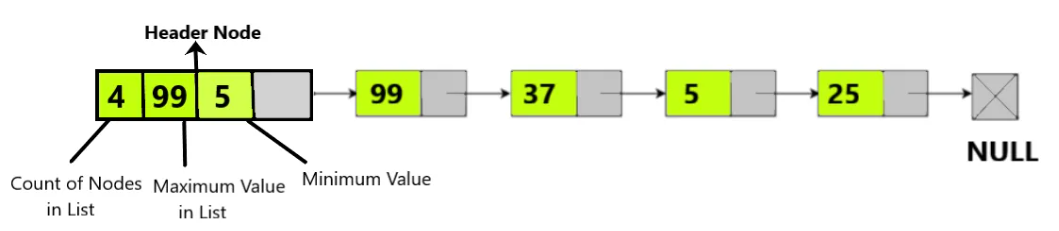
\includegraphics[width=0.8\textwidth]{figs/list/header_node_1.png}
\end{frame}

\begin{frame}[fragile]
  \frametitle{求表长}
  \begin{center}
    \scalebox{0.65}{
      \begin{tikzpicture}[fill=red, box/.style={draw, minimum width=0.85cm, minimum height=0.8cm, fill=red!5}]
	      \draw node[box, dashed] (h) {$hp$}
        node[box, thick, double, pattern=north west lines, right=of h] (d18) { }  node[box, thick, double, right=0 of d18] (p18) {}
        node[box, right=of p18] (d45) {45}  node[box, right=0 of d45] (p45) {}
        node[box, right=of p45] (d25) {25}  node[box, right=0 of d25] (p25) {$\wedge$}
	      node[below=1 of h] (tip1) {指向头节点的指针} node[below=1.5 of p18] (tip2) {头节点};
	      \path[draw, -Latex] (h) edge[-latex] (d18) (p18.center)  edge[-latex] (d45)  (p45.center) -- (d25);
	      \path (tip1) edge[draw=red,  thick, ->, out=45, in=270] (h) (tip2) edge[draw=red, thick, in=270, ->] (d18);
      \end{tikzpicture}
    }
  \end{center}

  \scriptsize
  \begin{columns}
    \begin{column}[T]{0.5\linewidth}
      \begin{minted}{c}
        int GetLength() {
          Node p= hp.next; // hp: head pointer
          int  len=0;
          while (p){
            p=p.next;
            len++;
          }
          return  len;
        }
      \end{minted}
    \end{column}
    \begin{column}[T]{0.5\linewidth}
      \pause
      \begin{minted}{python}
class Node:
    def __init__(self, data, next=None):
        self.data = data
        self.next = next

def get_length(hp):
    p = hp.next
    len = 0
    while(p!=None):
        p = p.next
        len = len + 1
    return len

hp = Node(None, Node(45, Node(25)))
print(get_length(hp))
      \end{minted}
    \end{column}
  \end{columns}
\end{frame}

\begin{frame}[fragile]
  \frametitle{单链表的查找}
  \begin{center}
    \scalebox{0.65}{
      \begin{tikzpicture}[fill=red, box/.style={draw, minimum width=0.85cm, minimum height=0.8cm, fill=red!5}]
	      \draw node[box, dashed] (h) {$hp$}
        node[box, thick, double, pattern=north west lines, right=of h] (d18) { }  node[box, thick, double, right=0 of d18] (p18) {}
        node[box, right=of p18] (d45) {45}  node[box, right=0 of d45] (p45) {}
        node[box, right=of p45] (d25) {25}  node[box, right=0 of d25] (p25) {$\wedge$};
	      \path[draw, -Latex] (h) edge[-latex] (d18) (p18.center)  edge[-latex] (d45)  (p45.center) -- (d25);
      \end{tikzpicture}
    }
  \end{center}

  \begin{itemize}
  \item 按值查找index(value): 是否存在数据元素X?序号是?
  \item 算法思路:“顺藤摸瓜”——从第一个结点开始,判断当前结点的值是否等于x,若是
    则返回该结点的指针,否则继续检查下一个,直到表尾。如果找不到则返回空。
  \end{itemize}

  \begin{minted}{c}
public int index(value){   //在L中查找值为x的结点
  Node  p=hp.next;  int j=0;
  while ( p && p.data !=value){
    p=p->next; j++;
  }
  if(p) return j; else return -1;
}
  \end{minted}
\end{frame}

\begin{frame}[fragile]
  \frametitle{插入新结点:在给定结点的前后}
  \begin{itemize}
  \item 新结点插入到p的后面
    \scalebox{0.65}{
      \begin{tikzpicture}[fill=red, box/.style={draw, minimum width=0.85cm, minimum height=0.8cm, fill=red!5}]
        \draw node[] (h) {}
        node[box, right=of h] (d1) { }  node[box, right=0 of d1] (p1) { ~ }
        node[box, right=of p1] (d2) {}  node[box, right=0 of d2] (p2) { ~ }
        node[box, right=3cm of p2] (d3) {}  node[box, right=0 of d3] (p3) {};

        \path[] (h.center) edge[-latex] (d1) (p1.center) edge[-latex] (d2) (p2.center) edge[draw, -Latex] node[color=red] {$\times$} (d3);

        \draw node[above right=of d1](p) {$p$};
        \draw[draw, -Latex] (p) --(d2);

        \draw node[below=of p2] (s) {$s$}
        node[box, right=of s] (ds) { }  node[box, right=0 of ds] (ps) { ~ };
        \draw[draw, -Latex] (s) --(ds);

        \path[] (p2.south) edge[draw=red, -Latex] node[below, align=center] {\textcircled{2}} (ds);
        \path[] (ps.center) edge[draw=red, -Latex, in=215] node[above, align=center] {\textcircled{1}} (d3);
      \end{tikzpicture}
    }

    \begin{minted}{c}
      s.next = p.next;
      p.next = s;
    \end{minted}

  \end{itemize}
\end{frame}

\begin{frame}[fragile]
  \frametitle{插入新结点:在给定结点的前后}
  \begin{itemize}
  \item 新结点插入到p的前面
    \scalebox{0.65}{
      \begin{tikzpicture}[fill=red, box/.style={draw, minimum width=0.85cm, minimum height=0.8cm, fill=red!5}]
        \draw node[] (h) {}
        node[box, right=of h] (d1) { }  node[box, right=0 of d1] (p1) { ~ }
        node[box, right=3cm of p1] (d2) {}  node[box, right=0 of d2] (p2) { ~ }
        node[box, right=of p2] (d3) {}  node[box, right=0 of d3] (p3) {};

        \path[] (h.center) edge[-latex] (d1) (p1.center) edge[-latex] node[color=red] {$\times$} (d2) (p2.center) edge[draw, -Latex]  (d3);

        \draw node[above left=of d2](p) {$p$};
        \draw[draw, -Latex] (p) --(d2);

        \draw node[above left=of d1](q) {$q$};
        \path (q)  edge[draw=red, -Latex] node[above] {\textcircled{1}} (d1);

        \draw node[below=of p1] (s) {$s$}
        node[box, right=of s] (ds) { }  node[box, right=0 of ds] (ps) { ~ };
        \draw[draw, -Latex] (s) --(ds);

        \path[] (p1.south) edge[draw=red, -Latex] node[below, align=center] {\textcircled{3}} (ds);
        \path[] (ps.center) edge[draw=red, -Latex, in=215] node[above, align=center] {\textcircled{2}} (d2);
      \end{tikzpicture}
    }

    找到p的前驱q,在q之后插入s。

    \begin{minted}{c}
q=head;
while (q.next!=p) q=q.next;
s.next=q.next;
q.next=s;
    \end{minted}
  \end{itemize}
\end{frame}

\begin{frame}[fragile]
  \frametitle{插入新结点}
  \begin{easylist}
    & 时间复杂度
    && 后插操作为$O(1)$: 不受$n$的影响
    && 前插操作因为要先找到$p$的前驱,时间性能为$O(n)$。

    \pause
    & 一个小技巧:
    && 将$s$插入到 $p$ 的后面,然后把$p.data$与$s.data$交换,这样能使得时间复杂性为$O(1)$。
  \end{easylist}
\end{frame}

\begin{frame}[fragile]
  \frametitle{删除结点}
  \begin{itemize}
  \item 删除p指向的结点 \\

    \scalebox{0.6}{
      \begin{tikzpicture}[fill=red, box/.style={draw, minimum width=0.85cm, minimum height=0.8cm, fill=red!5}]
        \draw node[] (h) {}
        node[box, right=of h] (d1) { }  node[box, right=0 of d1] (p1) { ~ }
        node[box, right=of p1] (d2) {}  node[box, right=0 of d2] (p2) { ~ }
        node[box, right=of p2] (d3) {}  node[box, right=0 of d3] (p3) {};

        \path[] (h.center) edge[-latex] (d1) (p1.center) edge[-latex] node[color=red] {$\times$} (d2) (p2.center) edge[draw, -Latex]  (d3);

        \draw node[above left=of d2](p) {$p$};
        \draw[draw, -Latex] (p) --(d2);

        \draw node[above left=of d1](q) {$q$};
        \path (q)  edge[draw=red, -Latex] node[above] {\textcircled{1}} (d1);

        \path (p1.south)  edge[draw=red, -Latex, in=240, out=300] node[above]{\textcircled{2}} (d3);
      \end{tikzpicture}
    }

    q.next=q.next.next;
  \item 首先要找到$p$的前驱结点$q$,其时间复杂性为$O(n)$。

  \item 若要删除$p$的后继结点(假设存在),则可以直接完成:\\
    p.next=p.next.next;
  \item 该操作的时间复杂性为$O(1)$ 。
  \end{itemize}
\end{frame}

\begin{frame}[fragile]
  \frametitle{删除第i个结点}
  \begin{minted}{c}
    int  Del(LinkList  L, int i)  //删除链表L第i个结点
    {
      p=get(L, i-1);  //查找第i-1个结点
      if (p==NULL) {
        printf("第i-1个结点不存在");   return -1;
      } else{
        if (!p->next)
          return 0; //第i个结点不存在
        else {
          p.next=p.next.next; //从链表中删除i
          return 1;
        }
      }
    }
  \end{minted}

  算法时间复杂度是$O(n)$
\end{frame}

\begin{frame}[fragile]
  \frametitle{单链表操作小结}
  \begin{itemize}
  \item 在单链表上当前结点之前插入、删除一个结点,必须知道其前驱结点。
  \item 单链表不具有按序号随机访问的特点,只能从头指针开始一个个顺序进行。
  \end{itemize}
\end{frame}

\begin{frame}[fragile]
  \frametitle{单循环链表}
  \begin{easylist}
    & 链表头尾结点相连

    \begin{center}
      \scalebox{0.65}{
        \begin{tikzpicture}[fill=red, box/.style={draw, minimum width=0.85cm, minimum height=0.8cm, fill=red!5}]
	        \draw node[box, dashed] (hp) {$hp$}
          node[box, thick, double, pattern=north west lines, right=of hp] (dh) { }  node[box, thick, double, right=0 of dh] (ph) {}
          node[box, right=of ph] (da1) {$a_1$}  node[box, right=0 of da1] (pa1) {}
          node[box, draw=none, right=of pa1] (dai) {$\cdots$}  node[box, draw=none,  right=0 of dai] (pai) {$\cdots$}
          node[box, right=of pai] (dan) {$a_n$}  node[box, right=0 of dan] (pan) {};

	        \path[draw, -Latex] (hp) edge[-latex] (dh) (ph.center)  edge[-Latex] (da1)
			    (pa1.center) edge[-Latex] (dai)
			    (pai.east) edge[-Latex] (dan)
			    (pan.center)  |- ++(0,-1) -| (dh);

          \draw node[box, dashed, right=1cm of pan] (hp) {$hp$}
          node[box, thick, double, pattern=north west lines, right=of hp] (dh) { }  node[box, thick, double, right=0 of dh] (ph) {};

          \path[draw, -Latex] (hp) edge[-latex] (dh) (ph.center)
			    (ph.center)  |- ++(0,-1) -| (dh);

          \draw node[below=1cm of pa1] {(a) 非空表} node[below=1cm of dh] {(b) 空表};
        \end{tikzpicture}
      }
    \end{center}

    & 结点的定义有什么变化?

    & 链表操作有什么变化?比如:

    && 原来用头结点的next是否为NULL (None)判断空表,现在呢?

    && 原来用结点的next是否为NULL (None)判断尾结点,现在呢?
  \end{easylist}
\end{frame}

\begin{frame}[fragile]
  \frametitle{双向链表}

  \begin{center}
    \scalebox{0.5}{
      \begin{tikzpicture}[fill=red, box/.style={draw, minimum width=0.85cm, minimum height=0.8cm, fill=red!5},
          e1/.style={draw=red, -Latex, in=160, out=30},
          e2/.style={draw=red, -Latex, in=-30, out=200}
        ]
	      \draw node[box, dashed] (hp) {$hp$}
		    node[box, thick, double,below right=of hp] (prevh) { }
        node[box, thick, double, pattern=north west lines, right=0 of prevh] (datah) { }  node[box, thick, double, right=0 of datah] (nexth) {}

		    node[box, right=of nexth] (prev1) {}   node[box, right=0 of prev1] (data1) {$a_1$}  node[box, right=0 of data1] (next1) {}

		    node[box, right=of next1] (prev2) {}   node[box, right=0 of prev2] (data2) {$a_2$}  node[box, right=0 of data2] (next2) {}

		    node[box, right=of next2, draw=none] (previ) {}   node[box, right=0 of previ, draw=none] (datai) {$\cdots$}  node[box, right=0 of datai, draw=none] (nexti) {}

		    node[box, right=of nexti] (prevn) {}   node[box, right=0 of prevn] (datan) {$a_n$}  node[box, right=0 of datan] (nextn) {};

        \path (hp) edge[out=0, -Latex, draw=blue] (prevh)
	      (nexth.center) edge[e1] (prev1)
        (next1.center) edge[e1] (prev2)
        (next2.center) edge[e1] (previ)
        (nexti.center) edge[e1] (prevn)
	      (prev1.center) edge[e2] (nexth)
        (prev2.center) edge[e2] (next1)
        (previ.center) edge[e2] (next2)
        (prevn.center) edge[e2] (nexti);

        \path[draw=red, thick, -Latex]  (nextn.center)  |- ++(0,-1) -| (prevh.240);
        \path[draw=red, thick, -Latex]  (prevh.center)  |- ++(0,1) -| (prevn.120);
      \end{tikzpicture}
    }

    \scriptsize (a) 有多个节点时的双向链表
  \end{center}

  \begin{columns}
    \begin{column}[T]{0.65\linewidth}
      \scriptsize
      \begin{itemize}
      \item 为什么需要双向链表?
      \item 在单链表中查找后继的时间性能是$O(1)$,查找前驱的时间性能是$O(n)$,如果也
        希望找前驱的时间性能达到$O(1)$,则需要在空间上付出代价 —— 每个结点再加一个指
        向前驱的指针域。
      \item 结点的定义和链表的操作有什么变化?

        \begin{minted}{java}
          class Node {
            Object data;
            Node prior, next;
          }
        \end{minted}
      \end{itemize}
    \end{column}
    \begin{column}[T]{0.35\linewidth}
      \begin{center}
        \scalebox{0.5}{
          \begin{tikzpicture}[fill=red, box/.style={draw, minimum width=0.85cm, minimum height=0.8cm, fill=red!5},
              e1/.style={draw=red, -Latex, in=160, out=30},
              e2/.style={draw=red, -Latex, in=-30, out=200}
            ]
	          \draw node[box, dashed] (hp) {$hp$}
		        node[box, thick, double, right=4cm of hp, yshift=-0.6cm] (prevh) { }
            node[box, thick, double, pattern=north west lines, right=0 of prevh] (datah) { }  node[box, thick, double, right=0 of datah] (nexth) {};

            \path[draw=blue, thick, -Latex]  (hp)  edge[out=0, in=180] (prevh.180);
            \path[draw=red, thick, -Latex]  (nexth.center)  |- ++(0,-1) -- ++(-4,0) |- (prevh.210);
            \path[draw=red, thick, -Latex]  (prevh.center)  |- ++(0,1) -- ++(-2,0)  |- (prevh.150);
          \end{tikzpicture}
        }

      \scriptsize (b) 只有头节点的情况
      \end{center}
    \end{column}
  \end{columns}
\end{frame}

\begin{frame}[fragile]
  \frametitle{链表特点}
  \begin{center}
    \scalebox{0.65}{
      \begin{tikzpicture}[fill=red, box/.style={draw, minimum width=0.85cm, minimum height=0.8cm, fill=red!5}]
	      \draw node[box] (h) {}
        node[box, thick, double, pattern=north west lines, right=of h] (d18) { }  node[box, thick, double, right=0 of d18] (p18) {}
        node[box, right=of p18] (d45) {45}  node[box, right=0 of d45] (p45) {}
        node[box, right=of p45] (d25) {25}  node[box, right=0 of d25] (p25) {$\wedge$};
	      \path[draw, -Latex] (h.center) edge[-latex] (d18) (p18.center)  edge[-latex] (d45)  (p45.center) -- (d25);
      \end{tikzpicture}
    }
  \end{center}

  \begin{easylist}
    & 优点

    && 插入删除方便

    && 动态分配

    \pause

    & 缺点

    && 随机访问效率低
  \end{easylist}
\end{frame}

\begin{frame}[fragile]
  \frametitle{顺序表 VS 链表}
  \begin{columns}
    \begin{column}[T]{0.5\linewidth}
      \begin{tcolorbox}[colframe=red, title=顺序表优点]
        \begin{itemize}
        \item 直观
        \item 随机访问效率高
        \item 没有为表达结点间的逻辑关系增加的额外开销
        \end{itemize}
      \end{tcolorbox}

      \begin{tcolorbox}[colframe=red, title=顺序表缺点]
        \begin{itemize}
        \item 插入删除时效率低
        \item 需要预先分配足够大的存储空间
        \end{itemize}
      \end{tcolorbox}
    \end{column}
    \begin{column}[T]{0.5\linewidth}
\begin{tcolorbox}[colframe=red, title=链表优点]
        \begin{itemize}
        \item 插入删除方便
        \item 动态分配
        \end{itemize}
      \end{tcolorbox}

      \begin{tcolorbox}[colframe=red, title=链表缺点]
        \begin{itemize}
        \item 为表达结点间的逻辑关系增加“指针域”
        \item 随机访问效率低
        \end{itemize}
      \end{tcolorbox}
    \end{column}
  \end{columns}
\end{frame}

\begin{frame}[fragile, allowframebreaks]
  \frametitle{选取恰当的存储结构}
  \begin{enumerate}
  \item 基于存储的考虑

    \begin{itemize}
    \item 使用顺序表,在程序执行之前要明确规定它的存储规模(对MAXSIZE要有合适的
      设定),过大造成浪费,过小造成溢出。可见对线性表的长度或存储规模难以估计时,
      不宜采用顺序表。
    \item 链表不用事先估计存储规模,但链表的存储密度较低。存储密度是指一个结点中
      数据元素所占的存储单元和整个结点所占的存储单元之比。显然链式存储结构的存储
      密度是小于1的。
    \end{itemize}

   \newpage

 \item 基于运算的考虑
   \begin{itemize}
   \item 在顺序表中按序号访问$a_i$的时间性能时$O(1)$,而链表中按序号访问的时间性
     能$O(n)$,所以如果经常做的运算是按序号访问数据元素,显然顺序表优于链表;
   \item 在顺序表中做插入、删除时平均移动表中一半的元素,如果数据元素的信息量较
     大且表较长,不可忽视这一点;
   \item 在链表中作插入、删除,虽然也要找插入位置,但操作主要是比较操作,从这个
     角度考虑优于顺序表。
   \end{itemize}

   \newpage

 \item 其它
   \begin{itemize}
   \item 顺序表容易实现,任何高级语言中都有数组类型,相对来讲简单直观,也是用户
     考虑的一个因素。
   \end{itemize}
  \end{enumerate}

  总之,两种存储结构各有长短,选择那一种由实际问题中的主要因素决定。通常“较稳定”
  的线性表选择顺序存储,而频繁做插入删除的话宜选择链式存储。
\end{frame}

\begin{frame}[fragile]
  \frametitle{本堂小结}
  \begin{enumerate}
  \item 线性表的概念和两种存储方式.
  \item 顺序线性表的特征、基本操作.
  \item 链表的特征、基本操作.
  \item 循环链表和双向链表
  \item 顺序表与链表大PK
  \item 顺序表和链表适用的场合
  \end{enumerate}
\end{frame}

\subsection{作业}
\begin{frame}[fragile]
  \frametitle{约瑟夫环}

  在罗马人占领乔塔帕特后,约瑟夫(Joseph)及他的40个战友躲到一个洞中,这些犹太人
  宁死也不想被敌人抓到,于是决定了一个自杀方式:

  \begin{itemize}
    \item 41个人排成一个圆圈,由第1个人开始报数,每报数到第3人该人就必须自杀,然
      后再由下一个重新报数,直到所有人都自杀身亡为止。
  \item 约瑟夫说他和另一个人逃过了这场死亡游戏: by luck or by the hand of God.
  \item 请问约瑟夫在这个圆圈中的位置是?
  \end{itemize}
\end{frame}

\begin{frame}[fragile]
  \frametitle{约瑟夫环}

  \begin{itemize}
  \item 已知$n$个人 (以编号$1, 2, 3 \cdots n$ 分别表示) 围坐在一张圆桌周围。从
    编号为$k$ 的人开始报数,数到$m$的那个人出列;他的下一个人又从1 开始报数,数
    到$m$的那个人又出列;依此规律重复下去,直到圆桌周围的人全部出列。

  \item 例如:n = 9, k = 1, m = 5;出局顺序如下

  \end{itemize}
  \begin{center}
    \scalebox{0.6} {
      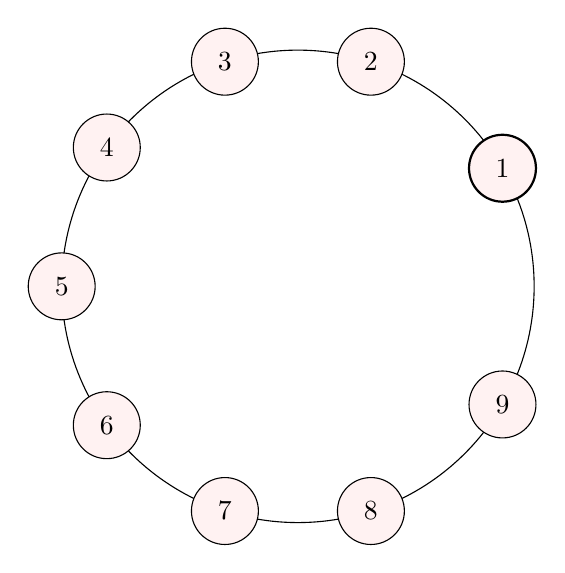
\begin{tikzpicture}[fill=red, ns/.style={draw, circle, minimum width=0.85cm, minimum height=0.8cm, fill=red!5}]
	      \node [draw, minimum size=6cm, circle] {};
        \node (n1) at (30:3cm) [ns, thick]   {1};
        \node (n2) at (72:3cm) [ns]   {2};
        \node (n3) at (108:3cm) [ns]   {3};
        \node (n4) at (144:3cm) [ns]   {4};
        \node (n5) at (180:3cm) [ns]   {5};
        \node (n6) at (216:3cm) [ns]   {6};
        \node (n7) at (252:3cm) [ns]   {7};
        \node (n8) at (288:3cm) [ns]   {8};
        \node (n9) at (330:3cm) [ns]   {9};
      \end{tikzpicture}
    }

    5, 1, 7, 4, 3, 6, 9, 2, 8
  \end{center}
\end{frame}

\begin{frame}[fragile]
  \frametitle{约瑟夫环动画演示}
  见PPT动画
\end{frame}
